\documentclass[border=8pt]{standalone}
\usepackage{tikz}
\usetikzlibrary{arrows.meta, positioning, calc}
\begin{document}
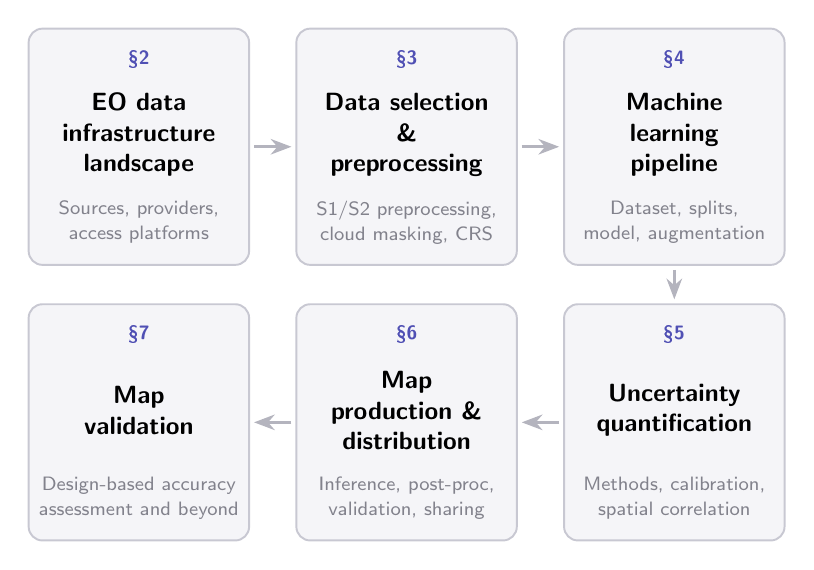
\begin{tikzpicture}[
    >=Stealth,
    every node/.style={font=\sffamily},
]
% Colors
\definecolor{accent}{RGB}{80,80,180}
\definecolor{boxfill}{RGB}{245,245,248}
\definecolor{boxstroke}{RGB}{200,200,210}
\definecolor{arrowgray}{RGB}{180,180,190}
\definecolor{subtextgray}{RGB}{130,130,140}
% ============================================================
% Styles
% ============================================================
\tikzset{
    stagebox/.style={
        draw=boxstroke,
        fill=boxfill,
        line width=0.7pt,
        rounded corners=5pt,
        minimum width=2.8cm,
        minimum height=3.0cm,
        inner sep=0pt,
    },
    title/.style={font=\sffamily\small\bfseries, align=center},
}
% ============================================================
% Six stage boxes — 3 columns x 2 rows, snake flow
% ============================================================
\def\gap{3.4}
\def\vgap{3.5}

% --- Top row (flow: left to right) ---
% Box 1: Data Landscape
\node[stagebox] (b1) at (0, 0) {};
\node[font=\sffamily\scriptsize\bfseries, accent] at ($(b1.north) + (0, -0.4)$) {\S2};
\node[title] at ($(b1.center) + (0, 0.15)$) {EO data\\infrastructure \\landscape};
\node[font=\sffamily\fontsize{7}{9}\selectfont, subtextgray, align=center] at ($(b1.south) + (0, 0.55)$) {Sources, providers,\\access platforms};
% Box 2: Selection & Processing
\node[stagebox] (b2) at (\gap, 0) {};
\node[font=\sffamily\scriptsize\bfseries, accent] at ($(b2.north) + (0, -0.4)$) {\S3};
\node[title] at ($(b2.center) + (0, 0.15)$) {Data selection \\ \& \\ preprocessing};
\node[font=\sffamily\fontsize{7}{9}\selectfont, subtextgray, align=center] at ($(b2.south) + (0, 0.55)$) {S1/S2 preprocessing,\\cloud masking, CRS};
% Box 3: ML Pipeline
\node[stagebox] (b3) at (2*\gap, 0) {};
\node[font=\sffamily\scriptsize\bfseries, accent] at ($(b3.north) + (0, -0.4)$) {\S4};
\node[title] at ($(b3.center) + (0, 0.15)$) {Machine\\learning\\pipeline};
\node[font=\sffamily\fontsize{7}{9}\selectfont, subtextgray, align=center] at ($(b3.south) + (0, 0.55)$) {Dataset, splits,\\model, augmentation};

% --- Bottom row (flow: right to left; positions mirror that) ---
% Box 4: Uncertainty Quantification (under b3)
\node[stagebox] (b4) at (2*\gap, -\vgap) {};
\node[font=\sffamily\scriptsize\bfseries, accent] at ($(b4.north) + (0, -0.4)$) {\S5};
\node[title] at ($(b4.center) + (0, 0.15)$) {Uncertainty\\quantification};
\node[font=\sffamily\fontsize{7}{9}\selectfont, subtextgray, align=center] at ($(b4.south) + (0, 0.55)$) {Methods, calibration,\\spatial correlation};
% Box 5: Map Generation (under b2)
\node[stagebox] (b5) at (\gap, -\vgap) {};
\node[font=\sffamily\scriptsize\bfseries, accent] at ($(b5.north) + (0, -0.4)$) {\S6};
\node[title] at ($(b5.center) + (0, 0.15)$) {Map\\production \& \\distribution};
\node[font=\sffamily\fontsize{7}{9}\selectfont, subtextgray, align=center] at ($(b5.south) + (0, 0.55)$) {Inference, post-proc,\\validation, sharing};
% Box 6: Validation (under b1)
\node[stagebox] (b6) at (0, -\vgap) {};
\node[font=\sffamily\scriptsize\bfseries, accent] at ($(b6.north) + (0, -0.4)$) {\S7};
\node[title] at ($(b6.center) + (0, 0.15)$) {Map\\validation};
\node[font=\sffamily\fontsize{7}{9}\selectfont, subtextgray, align=center] at ($(b6.south) + (0, 0.55)$) {Design-based accuracy \\assessment and beyond};

% ============================================================
% Arrows — snake flow: b1 -> b2 -> b3 -> b4 -> b5 -> b6
% ============================================================
% Top row, left to right
\foreach \i/\j in {b1/b2, b2/b3} {
    \draw[->, arrowgray, line width=1pt]
        ($(\i.east) + (0.05, 0)$) -- ($(\j.west) + (-0.05, 0)$);
}
% Vertical hop on the right: b3 -> b4
\draw[->, arrowgray, line width=1pt]
    ($(b3.south) + (0, -0.05)$) -- ($(b4.north) + (0, 0.05)$);
% Bottom row, right to left
\foreach \i/\j in {b4/b5, b5/b6} {
    \draw[->, arrowgray, line width=1pt]
        ($(\i.west) + (-0.05, 0)$) -- ($(\j.east) + (0.05, 0)$);
}
\end{tikzpicture}
\end{document}